% -------------------------------------------------------------------------------------- %

\section{Results}

The aforementioned parallelization techinques were tested using the Lorenz system 
\cite*{lorenz}

\begin{gather}
    \dot{x} = \sigma (y - x), \\
    \dot{y} = x (\rho - z) - y, \\
    \dot{z} = xy - \beta z,
\end{gather}

with the parameters $\sigma = 10,\ \rho = 28,\ \beta = 2 / 5$. The function $f_k$ was 
defined as performing $k$ steps of the classic fourth order Runge Kutta scheme with step 
size $1 / 10 k$. Further, the \jlinl{SampledBoxMap} \jlinl{Fₖᴺ} was generated to use $N$
Monte-Carlo test points to map boxes in a $128 \times 128 \times 128$-element equidisdant 
\jlinl{BoxPartition} over the compact domain 
$Q = [-30,30] \times [-30,30] \times [-5,55]$. \\

One trial of the test was calculating the unstable set for the equilibrium point 

\begin{equation}
    \label{eq:equilibrium}
    (x, y, z) = \left(\,\sqrt{\beta (\rho - 1)},\,\ \sqrt{\beta (\rho - 1)},\,\ \rho - 1\,\right)
\end{equation}

using \autoref{alg:manifold} (see also \autoref{lst:gum:julia}). The test was performed on 
a Dell G15 5510 laptop with Intel i7-10870H CPU and Nividia GeForce RTX 3060 laptop GPU, 
running Ubuntu 22.04 LTS. A depiction of the unstable set can be found in \autoref{fig:lorenz}, 
result graphs can be found in \autoref{fig:times}, and code for the tests can be found 
in \cite*{benchmarks}. \\

\begin{figure}
    \centering
    \makebox[\linewidth][c]{
        \begin{subfigure}[t]{0.6\textwidth}
            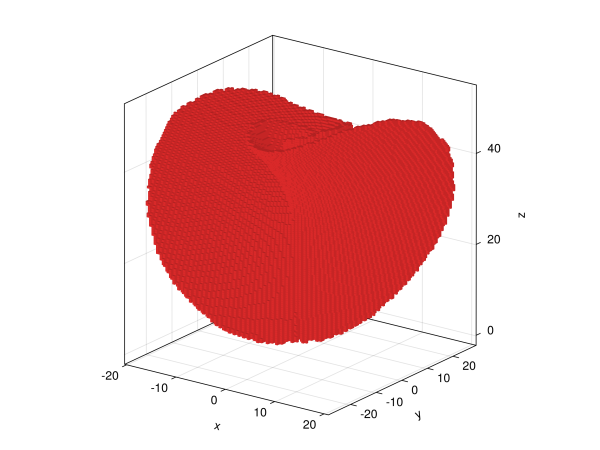
\includegraphics[width=0.95\textwidth]{lorenz1.pdf}
        \end{subfigure}
        \hfill
        \begin{subfigure}[t]{0.6\textwidth}
            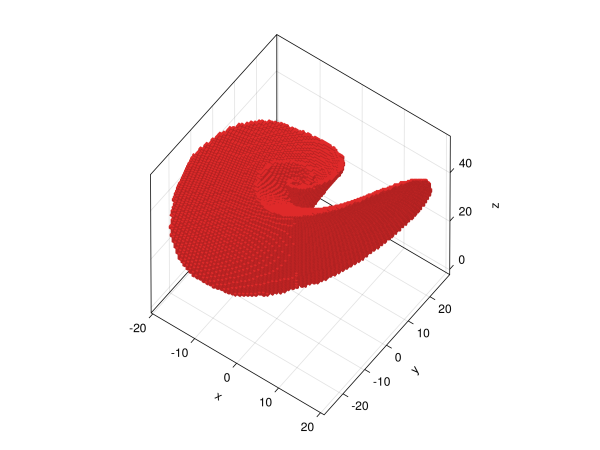
\includegraphics[width=0.95\textwidth]{lorenz2.pdf}
        \end{subfigure}
    }
    \\
    \makebox[\linewidth][c]{
        \begin{subfigure}[t]{0.6\textwidth}
            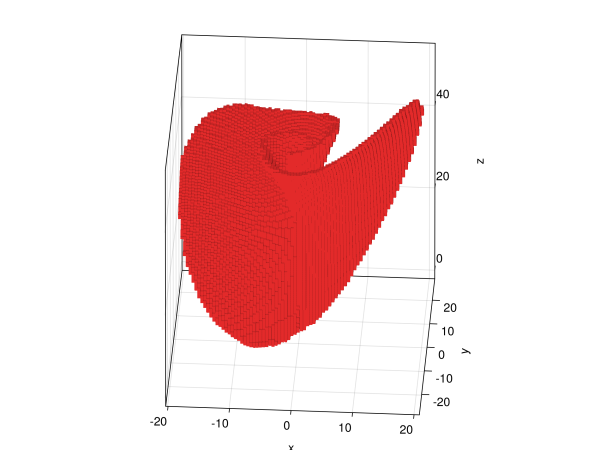
\includegraphics[width=0.95\textwidth]{lorenz3.pdf}
        \end{subfigure}
        \hfill
        \begin{subfigure}[t]{0.6\textwidth}
            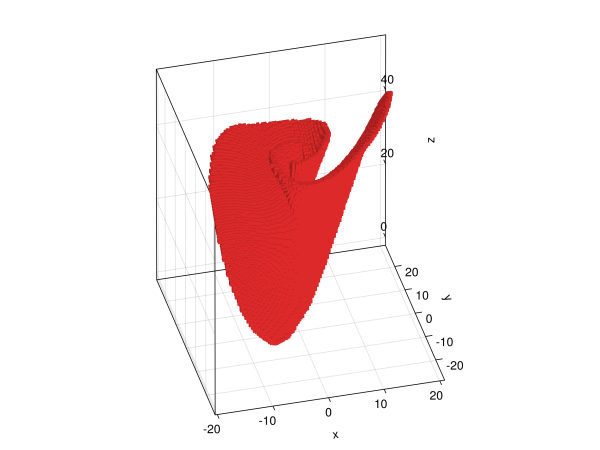
\includegraphics[width=0.95\textwidth]{lorenz4.pdf}
        \end{subfigure}
    }
    \caption{
        Box Covering of the unstable set for the Lorenz system around the equilibrium 
        point described in Eq. \ref{eq:equilibrium}
    }
    \label{fig:lorenz}
\end{figure}

\begin{figure}
    \centering
    \begin{subfigure}[t]{0.45\textwidth}
        \includegraphics[width=\textwidth]{times_simple.pdf}
        \caption{Times for a "simple" map, $k = 10$.}
        \label{fig:times:simple}
    \end{subfigure}
    \hfill
    \begin{subfigure}[t]{0.45\textwidth}
        \includegraphics[width=\textwidth]{times_medium.pdf}
        \caption{Times for an "average" map, $k = 100$.}
        \label{fig:times:med}
    \end{subfigure}
    \medskip
    \begin{subfigure}[t]{0.45\textwidth}
        \includegraphics[width=\textwidth]{times_simple_loglog.pdf}
        \caption{Log-Log plot of times for the "simple" map, $k = 10$.}
        \label{fig:times:simple:loglog}
    \end{subfigure}
    \hfill
    \begin{subfigure}[t]{0.45\textwidth}
        \includegraphics[width=\textwidth]{times_medium_loglog.pdf}
        \caption{Log-Log plot of times for the "average" map, $k = 100$.}
        \label{fig:times:med:loglog}
    \end{subfigure}
    \medskip
    \begin{subfigure}[t]{0.45\textwidth}
        \includegraphics[width=\textwidth]{times_complex_loglog.pdf}
        \caption{Log-Log plot of times for a "complex" map, $k = 1000$.}
        \label{fig:times:complex:loglog}
    \end{subfigure}
    \hfill
    \begin{subfigure}[t]{0.45\textwidth}
        \includegraphics[width=\textwidth]{times_steps_loglog.pdf}
        \caption{Log-Log plot of map complexity $k$ vs time, where $N = 400$ is constant.}
        \label{fig:times:steps:loglog}
    \end{subfigure}
    \caption{
        Execution time for \autoref{alg:manifold} using various steps $k$ and test points $N$. 
    }
    \label{fig:times}
\end{figure}

Execution time without acceleration and with CPU acceleration both show linear trends 
w.r.t. both $k$ and $N$. CPU acceleration consistently performs faster by a factor of 2 
across all trials. One might expect that the 256 bit vector registers, which can fit 4 
double-precision floating point numbers each, should provide a speedup factor of 4. 
A set of 4 double precision floating point multiplcations can be sped up by slightly less 
than a factor of 4 by replacing it with one packed SIMD multiplication. However, this does 
not factor in the time taken to convert the points into a vector stored in the YMM 
register (the gather and scatter operations). Furthermore, the bookkeeping required to 
manage a set of $d$-dimensional test vectors adds further complexity. Consider inlining 
the function \jlinl{tuple_vscatter!} (\autoref{lst:tuple_vscatter}) into the 
CPU-accelerated method for \jlinl{map_boxes} (\autoref{lst:boxmap}). The code length grows 
by nearly one third and includes an extra \jlinl{for} loop. \\

More interesting are the performance results of the GPU-accelerated code. Glancing at 
\autoref{fig:times:simple} it would seem that the GPU has actually hindered 
performance, though this is no longer the case in \autoref{fig:times:med}. This is 
because the calculation for the "simple" map can be performed so quickly that the 
execution time is dominated by the time it takes to transfer the box set to the GPU 
memory. A more detailed examination of this phenomenon can be seen in 
\autoref{fig:times:steps:loglog}. In this case $k = 26$ steps was required before the 
GPU-accelerated version beat out the version without acceleration, and $k = 32$ steps were 
required to beat the CPU-accelerated version. However, once this threshold has been 
passed the GPU performs significantly better. Moreover, the speedup factor does not remain 
bounded, as it did with the CPU version. By $k = 7944$ steps, the GPU version has 
surpassed a 100-fold speedup, and continues to climb. Due to the limits of the testing 
hardware and time, steps were only tested up to $k = 10000$. At this point the rate of 
increase of the speedup factor had slowed, though notably had not stopped. \\

The results of the present paper solidify that GAIO.jl is a perfect candidate for 
parallel programming due to its high proportion of data-independent computations. As of 
the writing, there are still regions of active development. These include endowing the 
matrix transfer operator $P_{ij}$ from \autoref{eq:pij} with a structure that allows it to 
act as the approximate transfer operator $Q_n P$ from \autoref{eq:qnp}, as well as 
efficiently porting adaptive test point sampling techniques to the GPU. 

% -------------------------------------------------------------------------------------- %
